\subsubsection{Analytics}

\begin{center}
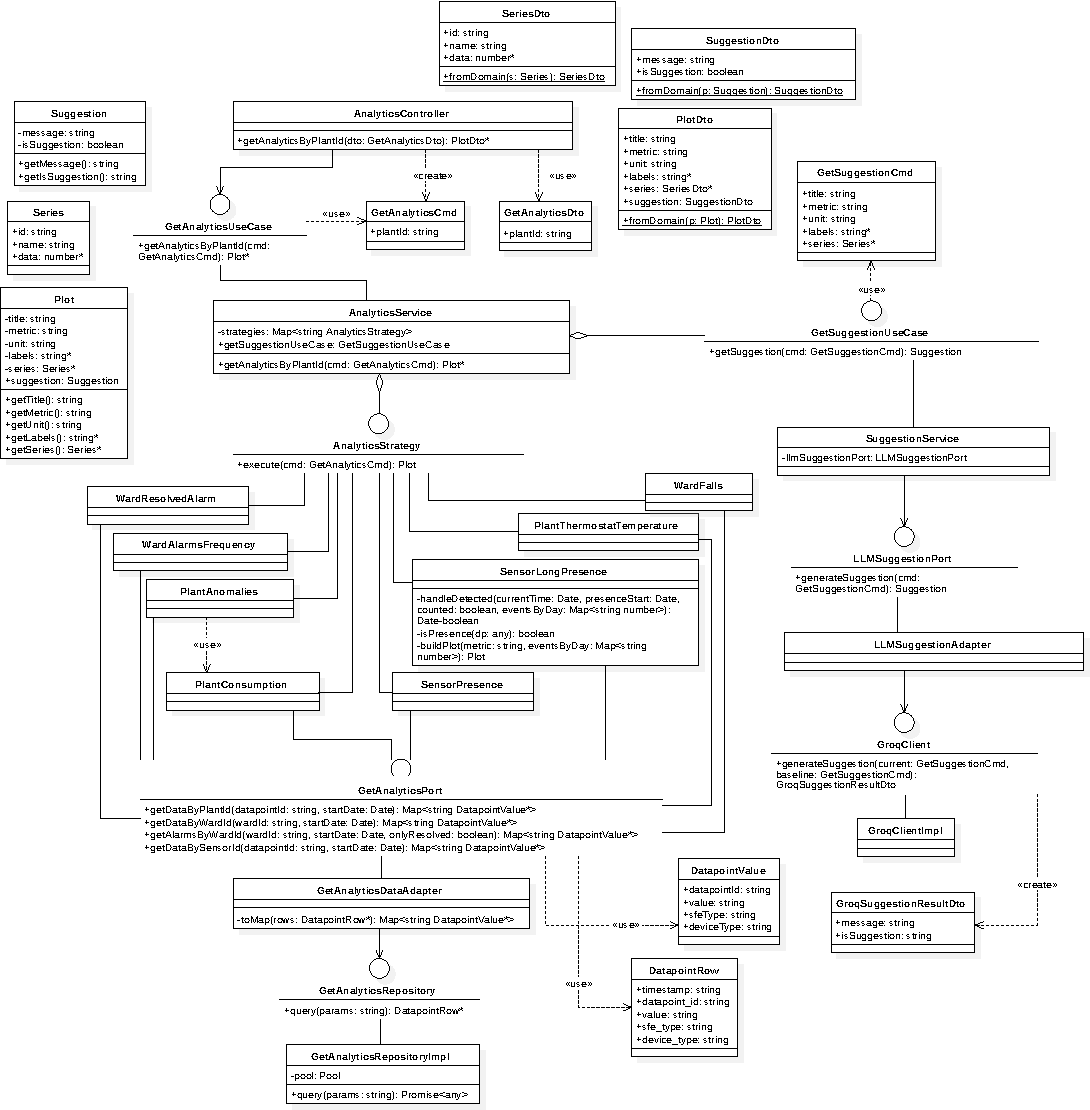
\includegraphics[width=\textwidth]{./backend/analytics/analytics.pdf}
\captionof{figure}{\href{https://snakebyteteam.github.io/3-PB/Documenti_esterni/Specifica_tecnica/backend/analytics/analytics.pdf}{Diagramma delle classi del modulo Analytics}}
\end{center}

% ─── infrastructure/dtos ───
\addAtr{+}{plantId: string}{Identificativo dell'impianto (appartamento) per cui richiedere le analytics}
\makeCl{GetAnalyticsDto}{DTO di input per l'endpoint REST. Trasporta l'identificativo dell'impianto ricevuto nella richiesta HTTP verso il controller, che lo converte in un \texttt{GetAnalyticsCmd}.}
\addAtr{+}{title: string}{Titolo del plot}
\addAtr{+}{metric: string}{Nome della metrica rappresentata}
\addAtr{+}{unit: string}{Unità di misura della metrica}
\addAtr{+}{labels: string[]}{Etichette temporali del grafico}
\addAtr{+}{series: SeriesDto[]}{Serie di dati serializzate per il trasporto via API}
\addAtr{+}{suggestion: SuggestionDto $|$ undefined}{Suggerimento energetico serializzato, se presente}
\addMet{+}{fromDomain(plot: Plot) : PlotDto}{Costruisce il DTO a partire dall'oggetto di dominio Plot}
\makeCl{PlotDto}{DTO di output che serializza un oggetto \texttt{Plot} per il trasporto via API REST. Espone il metodo factory \texttt{fromDomain} per la conversione dall'entità di dominio, includendo opzionalmente il \texttt{SuggestionDto}.}
\addAtr{+}{id: string}{Identificativo univoco della serie}
\addAtr{+}{name: string}{Nome descrittivo della serie}
\addAtr{+}{data: number[]}{Valori numerici della serie}
\addMet{+}{fromDomain(series: Series) : SeriesDto}{Costruisce il DTO a partire dall'oggetto di dominio Series}
\makeCl{SeriesDto}{DTO di output che serializza un oggetto \texttt{Series}. Espone il metodo factory \texttt{fromDomain} e riproduce i campi \texttt{id}, \texttt{name} e \texttt{data} in forma piatta adatta alla serializzazione JSON.}
\addAtr{+}{message: string[]}{Messaggi testuali del suggerimento}
\addAtr{+}{isSuggestion: boolean}{Indica se è presente un suggerimento effettivo}
\addMet{+}{fromDomain(suggestion: Suggestion) : SuggestionDto}{Costruisce il DTO a partire dall'oggetto di dominio Suggestion}
\makeCl{SuggestionDto}{DTO di output che serializza un oggetto \texttt{Suggestion}. Espone il metodo factory \texttt{fromDomain} e trasporta i messaggi e il flag \texttt{isSuggestion} verso il client.}
% ─── adapters/in ───
\addAtr{-}{getAnalyticsUseCase: GetAnalyticsUseCase}{Use case per il recupero delle analytics di un impianto}
\addMet{+}{getAnalyticsByPlantId: GetAnalyticsDto}{Riceve l'identificativo dell'impianto dalla richiesta HTTP, costruisce un \texttt{GetAnalyticsCmd} e delega al \texttt{GetAnalyticsUseCase}, restituendo la lista di \textsl{PlotDto} serializzati}
\makeCl{AnalyticsController}{Controller REST che espone l'endpoint per il recupero delle analytics di un impianto. Riceve la richiesta HTTP, la delega al \texttt{GetAnalyticsUseCase} e restituisce al client la lista di plot e relativi suggerimenti serializzati come DTO.}
% ─── application/commands ───
\addAtr{+}{plantId: string}{Identificativo dell'impianto (appartamento) da cui recuperare le analytics}
\makeCl{GetAnalyticsCmd}{Comando applicativo che trasporta l'identificativo dell'impianto necessario per avviare il recupero delle analytics.}
\addAtr{+}{title: string}{Titolo della metrica da analizzare}
\addAtr{+}{metric: string}{Nome della metrica oggetto del confronto con la baseline}
\addAtr{+}{unit: string}{Unità di misura della metrica}
\addAtr{+}{labels: string[]}{Etichette temporali dell'asse x del grafico}
\addAtr{+}{series: Series[]}{Serie di dati dell'analytics corrente da confrontare con la baseline. Corrispondono ai valori dell'asse y del grafico}
\makeCl{GetSuggestionCmd}{Comando applicativo che racchiude tutti i dati necessari alla generazione di un suggerimento.}
% ─── application/ports/in ───
\addMet{+}{getAnalyticsByPlantId(cmd: GetAnalyticsCmd) : Promise$<$Plot[]$>$}{Restituisce tutte le analytics disponibili per l'impianto identificato dal comando}
\makeItf{GetAnalyticsUseCase}{Porta di ingresso (driving port) che definisce il contratto per il recupero delle analytics di un impianto. Espone il metodo \texttt{getAnalyticsByPlantId}, implementato da \texttt{AnalyticsService}.}
\addMet{+}{getSuggestion(cmd: GetSuggestionCmd) : Promise$<$Suggestion$>$}{Richiede la generazione di un suggerimento per il risparmio energetico confrontando l'analytics corrente con la baseline}
\makeItf{GetSuggestionUseCase}{Porta di ingresso che definisce il contratto per la generazione di suggerimenti energetici tramite LLM. Espone il metodo \texttt{getSuggestion}, implementato da \texttt{SuggestionService}.}
% ─── application/services ───
\addAtr{-}{strategies: Map$<$string, AnalyticsStrategy$>$}{Mappa delle strategie di analytics disponibili, indicizzate per nome}
\addAtr{-}{getSuggestionUseCase: GetSuggestionUseCase}{Use case per la generazione di suggerimenti energetici tramite LLM}
\addMet{+}{getAnalyticsByPlantId(cmd: GetAnalyticsCmd) : Promise$<$Plot[]$>$}{Esegue tutte le strategie di analytics registrate per l'impianto e aggrega i risultati in una lista di plot}
\makeCl{AnalyticsService}{Servizio applicativo che implementa \texttt{GetAnalyticsUseCase}. Itera su tutte le strategie di analytics registrate nella mappa \texttt{strategies}, le esegue per l'impianto richiesto, genera i suggerimenti e aggrega i plot risultanti in una lista da restituire al controller.}
\addAtr{-}{llmSuggestionPort: LLMSuggestionPort}{Porta verso l'adapter LLM per la generazione di suggerimenti}
\addMet{+}{getSuggestion(cmd: GetSuggestionCmd) : Promise$<$Suggestion$>$}{Delega al modello LLM il confronto tra analytics corrente e baseline e restituisce i suggerimenti generati, se presenti}
\makeCl{SuggestionService}{Servizio applicativo che implementa \texttt{GetSuggestionUseCase}. Riceve il comando con i dati dell'analytics corrente e delega interamente al modello LLM — tramite \texttt{LLMSuggestionPort} — il confronto con la baseline e la generazione del suggerimento.}
% ─── application/ports/out ───
\addMet{+}{getDataForPlant(plantId: string, startDate: Date) : \\ Promise$<$Map$<$string, DatapointValue[]$>$$>$}{Recupera dal database i datapoint dell'impianto identificato da \texttt{plantId} a partire da \texttt{startDate}, restituendoli come mappa indicizzata per timestamp}
\addMet{+}{getDataForWard(wardId: string, startDate: Date) : \\ Promise$<$Map$<$string, DatapointValue[]$>$$>$}{Recupera dal database i datapoint di tutti gli impianti del reparto identificato da \texttt{wardId} a partire da \texttt{startDate}, restituendoli come mappa indicizzata per timestamp}
\addMet{+}{getAlarmsForWard(wardId: string, startDate: Date, onlyResolved: boolean) : \\ Promise$<$Map$<$string, number$>$$>$}{Recupera dal database gli allarmi del reparto identificato da \texttt{wardId} a partire da \texttt{startDate}; se \texttt{onlyResolved} è true, filtra i soli allarmi risolti}
\addMet{+}{getDataForSensor(sensorId: string, startDate: Date) : \\ Promise$<$Map$<$string, DatapointValue[]$>$$>$}{Recupera dal database i datapoint del sensore identificato da \texttt{sensorId} a partire da \texttt{startDate}, restituendoli come mappa indicizzata per timestamp}
\makeItf{GetAnalyticsPort}{Porta di uscita (driven port) che definisce il contratto per l'interrogazione dei datapoint sul database. Espone metodi specializzati per il recupero dei dati per impianto, reparto, allarmi di reparto e singolo sensore. Viene implementata da \texttt{GetAnalyticsData}.}
\addMet{+}{generateSuggestion(cmd: GetSuggestionCmd) : Promise$<$Suggestion$>$}{Invia i dati dell'analytics corrente e della baseline al modello LLM e restituisce eventuali suggerimenti per il risparmio energetico}
\makeItf{LLMSuggestionPort}{Porta di uscita che definisce il contratto per la comunicazione con il modello LLM. Espone \texttt{generateSuggestion}, implementata da \texttt{LLMSuggestionAdapter}.}
% ─── domain ───
\addAtr{-}{title: string}{Titolo del grafico dell'analytics}
\addAtr{-}{metric: string}{Nome della metrica rappresentata}
\addAtr{-}{unit: string}{Unità di misura della metrica}
\addAtr{-}{labels: string[]}{Etichette dell'asse temporale del grafico}
\addAtr{-}{series: Series[]}{Serie di dati che compongono il grafico}
\addAtr{-}{suggestion: Suggestion}{Suggerimento energetico associato al plot, se generato dal modello LLM}
\addMet{+}{getTitle() : string}{Restituisce il titolo del plot}
\addMet{+}{getMetric() : string}{Restituisce il nome della metrica rappresentata}
\addMet{+}{getUnit() : string}{Restituisce l'unità di misura della metrica}
\addMet{+}{getLabels() : string[]}{Restituisce le etichette dell'asse temporale}
\addMet{+}{getSeries() : Series[]}{Restituisce le serie di dati del plot}
\addMet{+}{getSuggestion() : Suggestion $|$ undefined}{Restituisce il suggerimento energetico associato al plot, se presente}
\addMet{+}{setSuggestion(s: Suggestion) : void}{Associa un suggerimento energetico al plot}
\makeCl{Plot}{Entità di dominio che rappresenta un grafico analytics completo. Aggrega titolo, metrica, unità, etichette temporali, serie di dati e, opzionalmente, un suggerimento LLM associato. Espone getter per tutti i campi e un setter per il suggerimento.}
\addAtr{-}{id: string}{Identificativo univoco della serie}
\addAtr{-}{name: string}{Nome descrittivo della serie (es. nome del sensore)}
\addAtr{-}{data: number[]}{Valori numerici della serie, allineati alle etichette del plot}
\addMet{+}{getId() : string}{Restituisce l'identificativo della serie}
\addMet{+}{getName() : string}{Restituisce il nome della serie}
\addMet{+}{getData() : number[]}{Restituisce i valori numerici della serie}
\makeCl{Series}{Value object di dominio che rappresenta una singola serie di dati all'interno di un \texttt{Plot}. Contiene un identificativo, un nome descrittivo e l'array di valori numerici allineati alle etichette temporali del plot padre.}
\addAtr{-}{message: string[]}{Lista di messaggi testuali che compongono il suggerimento generato dal modello LLM}
\addAtr{-}{isSuggestion: boolean}{Indica se il modello LLM ha rilevato un problema e ha generato un suggerimento effettivo}
\addMet{+}{getMessage() : string[]}{Restituisce i messaggi del suggerimento}
\addMet{+}{getIsSuggestion() : boolean}{Restituisce true se è presente un suggerimento effettivo generato dal modello}
\makeCl{Suggestion}{Value object di dominio che incapsula il risultato della generazione LLM: una lista di messaggi testuali e un flag booleano che distingue tra una risposta generica e un suggerimento effettivo basato su un'anomalia rilevata.}
% ─── adapters/out ───
\addAtr{-}{repository: GetAnalyticsRepositoryPort}{Repository per l'esecuzione di query sui datapoint}
\addAtr{+}{plantId: string}{Identificativo dell'impianto (appartamento) da cui recuperare i dati}
\addAtr{+}{startDate: Date}{Data di inizio del periodo di analisi}
\addAtr{+}{wardId: string}{Identificativo del reparto a cui appartiene l'impianto}
\addAtr{+}{onlyResolved: boolean}{Se true, filtra i soli allarmi risolti}
\addMet{-}{toMap(rows: DatapointRow[]) : Map$<$string, DatapointValue[]$>$}{Converte una lista di righe grezze di datapoint in una mappa indicizzata per timestamp ISO}
\makeCl{GetAnalyticsData}{Adapter che implementa la porta \texttt{GetAnalyticsPort}. Si occupa di richiamare \\ \texttt{GetAnalyticsRepositoryImpl}, convertendo le righe grezze restituite in mappe di \texttt{DatapointValue} indicizzate per timestamp tramite il metodo \texttt{toMap}.}
\addAtr{-}{groqClient: GroqClient}{Client per la comunicazione con le API Groq (modello LLaMA 3.3)}
\addMet{+}{generateSuggestion(cmd: GetSuggestionCmd) : Promise$<$Suggestion$>$}{Inoltra la richiesta di generazione suggerimento al client Groq e restituisce il risultato}
\makeCl{LLMSuggestionAdapter}{Adapter che implementa la porta \texttt{LLMSuggestionPort}. Fa da ponte tra il dominio applicativo e le API Groq, inoltrando i dati dell'analytics corrente al modello LLaMA 3.3 e restituendo il suggerimento generato come oggetto \texttt{Suggestion}.}
% ─── application/repository ───
\addMet{+}{query(sql: string) : Promise$<$DatapointRow[] $|$ any[]$>$}{Esegue una query SQL sul database e restituisce le righe risultanti}
\makeItf{GetAnalyticsRepositoryPort}{Porta di uscita di basso livello che astrae l'accesso diretto al database. Definisce il metodo \texttt{query} per l'esecuzione di SQL grezzo, implementato da \texttt{GetAnalyticsRepositoryImpl}.}
% ─── infrastructure/persistence ───
\addAtr{-}{pool: Pool}{Pool di connessioni al database}
\addMet{+}{query(sql: string) : Promise$<$any$>$}{Esegue una query SQL sul database tramite il pool di connessioni e restituisce i risultati grezzi}
\makeCl{GetAnalyticsRepositoryImpl}{Implementazione concreta di \texttt{GetAnalyticsRepositoryPort}. Gestisce un pool di connessioni e delega l'esecuzione delle query SQL al pool, restituendo i risultati grezzi allo strato applicativo.}
% ─── application/strategy ───
\addMet{+}{execute(cmd: GetAnalyticsCmd) : Promise$<$Plot$>$}{Esegue la strategia di analytics e restituisce il plot risultante}
\makeItf{AnalyticsStrategy}{Interfaccia che definisce il contratto del pattern Strategy per le analytics. Ogni strategia concreta implementa \texttt{execute}, che riceve un \texttt{GetAnalyticsCmd} e restituisce un \texttt{Plot}.}
% ─── application/strategy/strategies ───
\addMet{+}{execute(cmd: GetAnalyticsCmd) : Promise$<$Plot$>$}{Conta le anomalie di consumo energetico dell'impianto: un valore viene considerato anomalo se supera una soglia elevata rispetto ai valori di PlantConsumption}
\makeCl{PlantAnomalies}{Strategia che analizza i consumi energetici dell'impianto e conta i valori anomali, ovvero quelli che superano una soglia elevata rispetto ai valori restituiti da \texttt{PlantConsumption}. Restituisce un plot con il numero di anomalie aggregate nel periodo.}
\addAtr{-}{analyticsPort: GetAnalyticsPort}{Porta per il recupero dei dati di consumo energetico dell'impianto dal DB}
\addMet{+}{execute(cmd: GetAnalyticsCmd) : Promise$<$Plot$>$}{Calcola e restituisce il plot del consumo energetico dell'impianto nel periodo richiesto}
\makeCl{PlantConsumption}{Strategia che recupera i dati di consumo energetico dell'impianto tramite \texttt{GetAnalyticsPort} e restituisce il plot dei consumi nel periodo richiesto. Funge anche da riferimento per la rilevazione delle anomalie in \texttt{PlantAnomalies}.}
\addAtr{-}{analyticsPort: GetAnalyticsPort}{Porta per il recupero dei dati di temperatura dei termostati dell'impianto dal DB}
\addMet{+}{execute(cmd: GetAnalyticsCmd) : Promise$<$Plot$>$}{Calcola e restituisce il plot delle temperature rilevate dai termostati dell'impianto nel periodo richiesto}
\makeCl{PlantThermostatTemperature}{Strategia che recupera le temperature rilevate dai termostati dell'impianto tramite \texttt{GetAnalyticsPort} e le aggrega in un plot temporale, utile per analizzare l'andamento termico degli appartamenti.}
\addAtr{-}{analyticsPort: GetAnalyticsPort}{Porta per il recupero degli snapshot di stato dei sensori di presenza dal DB}
\addAtr{+}{snapshotsMap: Map$<$string, DatapointValue[]$>$}{Mappa degli snapshot di stato dei sensori, indicizzata per timestamp}
\addAtr{+}{sensorState: Map$<$string, SensorState$>$}{Stato corrente di ciascun sensore di presenza, indicizzato per ID sensore}
\addAtr{+}{sensorId: string}{Identificativo del sensore di presenza in elaborazione}
\addAtr{+}{name: string}{Nome del sensore di presenza in elaborazione}
\addAtr{+}{currentTime: Date}{Timestamp corrente durante la scansione degli snapshot}
\addAtr{+}{presenceStart: Date $|$ undefined}{Timestamp di inizio della presenza prolungata in corso, se attiva}
\addAtr{+}{counted: boolean}{Indica se la presenza prolungata corrente è già stata conteggiata}
\addAtr{+}{eventsByDay: Map$<$string, number$>$}{Numero di presenze prolungate (oltre 30 minuti) rilevate per ciascun giorno}
\addAtr{+}{labels: string[]}{Etichette dei giorni usate come asse x del plot finale}
\addAtr{+}{seriesMap: Map$<$string, $>$}{Mappa delle serie dati per ciascun sensore, usata per costruire il plot}
\addMet{+}{execute(cmd: GetAnalyticsCmd) : Promise$<$Plot$>$}{Rileva le presenze prolungate (oltre 30 minuti) contando i cambi di stato dei sensori e restituisce il plot aggregato per giorno}
\addMet{-}{getStartDate() : Date}{Calcola la data di inizio del periodo di analisi a partire dalla configurazione del comando}
\addMet{-}{emptyPlot() : Plot}{Restituisce un plot vuoto da usare come fallback in assenza di dati}
\makeCl{SensorLongPresence}{Strategia che rileva le presenze prolungate (oltre 30 minuti).}
\addAtr{-}{analyticsPort: GetAnalyticsPort}{Porta per il recupero dei valori dei sensori di presenza dal DB}
\addAtr{+}{sensorState: Map$<$string, SensorState$>$}{Stato corrente di ciascun sensore, indicizzato per ID sensore}
\addAtr{+}{sensorId: string}{Identificativo del sensore di presenza in elaborazione}
\addAtr{+}{name: string}{Nome del sensore di presenza in elaborazione}
\addMet{+}{execute(cmd: GetAnalyticsCmd) : Promise$<$Plot$>$}{Rileva le presenze leggendo direttamente i valori forniti dai datapoint dei sensori e restituisce il plot aggregato per giorno}
\makeCl{SensorPresence}{Strategia che rileva le presenze leggendo direttamente i valori forniti dai datapoint dei sensori.}
\addAtr{-}{analyticsPort: GetAnalyticsPort}{Porta per il recupero dei dati di allarme del reparto dal DB}
\addMet{+}{execute(cmd: GetAnalyticsCmd) : Promise$<$Plot$>$}{Calcola la frequenza degli allarmi inviati nel reparto (indipendentemente dalla risoluzione) aggregata per giorno}
\makeCl{WardAlarmsFrequency}{Strategia che calcola la frequenza giornaliera degli allarmi inviati nel reparto, indipendentemente dal loro stato di risoluzione. Recupera i dati tramite \texttt{GetAnalyticsPort} e li aggrega in un plot di frequenza per giorno.}
\addAtr{-}{analyticsPort: GetAnalyticsPort}{Porta per il recupero degli eventi di caduta rilevati nel reparto dal DB}
\addMet{+}{execute(cmd: GetAnalyticsCmd) : Promise$<$Plot$>$}{Conta e restituisce il plot degli eventi di caduta rilevati dai sensori negli appartamenti del reparto, aggregati per giorno}
\makeCl{WardFalls}{Strategia che conta gli eventi di caduta rilevati dai sensori negli appartamenti del reparto. Recupera gli eventi tramite \texttt{GetAnalyticsPort} e restituisce un plot con il numero di cadute aggregate per giorno.}
\addAtr{-}{analyticsPort: GetAnalyticsPort}{Porta per il recupero degli allarmi del reparto dal DB}
\addMet{+}{execute(cmd: GetAnalyticsCmd) : Promise$<$Plot$>$}{Traccia per il reparto il numero di allarmi totali e il numero di allarmi risolti, aggregati per giorno}
\makeCl{WardResolvedAlarm}{Strategia che traccia, per ciascun giorno del periodo analizzato, sia il totale degli allarmi del reparto sia il sottoinsieme di quelli risolti, consentendo di valutare il tasso di risoluzione nel tempo.}
% ─── infrastructure/groq ───
\addMet{+}{generateSuggestion(current: GetSuggestionCmd, baseline: GetSuggestionCmd) : \\ Promise$<$GroqSuggestionResultDto$>$}{Effettua la chiamata al LLM per generare i suggerimenti a partire dai dati correnti e di baseline}
\makeItf{GroqClient}{Interfaccia che definisce il contratto del client Groq. Dichiara i campi \texttt{current} e \texttt{baseline} come dati di input per la generazione del suggerimento, implementata da \texttt{GroqClientImpl}.}

\addAtr{-}{apiKey: string}{Chiave API per l'autenticazione verso il servizio Groq}
\addAtr{-}{apiUrl: string}{URL dell'endpoint Groq per la generazione di completamenti}
\addAtr{-}{model: string}{Identificativo del modello LLaMA utilizzato per la generazione}
\addMet{+}{generateSuggestion(current: GetSuggestionCmd, baseline: GetSuggestionCmd) : \\ Promise$<$GroqSuggestionResultDto$>$}{Invia il prompt costruito a partire dai dati correnti e di baseline all'API Groq e restituisce il suggerimento parsato; in caso di metrica non supportata, serie vuote, errore HTTP o risposta malformata restituisce un suggerimento vuoto}
\addMet{-}{buildPrompt(current: GetSuggestionCmd, baseline: GetSuggestionCmd) : string}{Costruisce il prompt completo da inviare al modello, includendo contesto stagionale, descrizione della metrica e la sezione statistica appropriata (scalare o per serie)}
\addMet{-}{buildScalarStatistics(current: GetSuggestionCmd, baseline: GetSuggestionCmd) : \\ string}{Produce la sezione statistica del prompt per metriche scalari: per la temperatura include il range accettabile dalla baseline, per le altre metriche calcola media corrente, media baseline e deviazione percentuale}
\addMet{-}{buildScalarInstructions(metric: string) : string}{Costruisce le istruzioni comportamentali del prompt per metriche scalari, differenziando le soglie e le azioni suggerite in base alla metrica specifica}
\addMet{-}{buildSeriesStatistics(current: GetSuggestionCmd, baseline: GetSuggestionCmd) : \\ string}{Produce la sezione statistica del prompt per metriche multi-sensore, calcolando per ciascuna serie la media corrente, la media baseline e la deviazione percentuale}
\addMet{-}{buildSeriesInstructions() : string}{Costruisce le istruzioni comportamentali del prompt per metriche multi-sensore, richiedendo al modello di analizzare ogni sensore individualmente e segnalare deviazioni oltre il 30\%}
\addMet{-}{rangeFromBaseline(baseline: GetSuggestionCmd) : \{min: number, max: number\}}{Estrae il valore minimo e massimo dalla prima serie della baseline, usati come range accettabile per la metrica temperatura}
\addMet{-}{averageFromLabels(cmd: GetSuggestionCmd) : number}{Calcola la media aritmetica dei valori numerici validi contenuti nella prima serie del comando}
\addMet{-}{averageFromData(data: number[]) : number}{Calcola la media aritmetica di un array di valori numerici}
\addMet{-}{deviationBetween(current: number, baseline: number) : string}{Calcola e formatta la deviazione percentuale del valore corrente rispetto alla baseline; restituisce \texttt{"0.0"} se la baseline è zero}
\makeCl{GroqClientImpl}{Implementazione concreta di \texttt{GroqClient}. Costruisce prompt contestualizzati (stagione, metrica, statistiche) e li invia al modello LLaMA 3.3 tramite le API Groq. Gestisce sia metriche scalari che multi-sensore, validando la risposta JSON prima di restituirla; in caso di errore o risposta non conforme restituisce un suggerimento vuoto.}